\documentclass{beamer}

\usepackage[T1]{fontenc}

	% é è à ...
\usepackage[utf8]{inputenc}
\usepackage[french]{babel}

	% Cosmetique :D
\usepackage{color}
\usepackage{url}
\usepackage{caption}
\usepackage{tcolorbox}
\usepackage{xcolor}
\usepackage{multicol}

	% Images
\usepackage{graphicx}
\usepackage{float}

	% Maths/phy
\usepackage[squaren,Gray]{SIunits}
\usepackage{amssymb}
\usepackage{amsmath}
\usepackage{mathtools}
\usepackage{physics}

	% Biblio
\usepackage{cite}


	% integration prog
\usepackage{listings}

\definecolor{mygreen}{rgb}{0,0.6,0}
\definecolor{mygray}{rgb}{0.5,0.5,0.5}
\definecolor{mymauve}{rgb}{0.58,0,0.82}
\lstset{ %
  backgroundcolor=\color{white},   % choose the background color; you must add \usepackage{color} or \usepackage{xcolor}; should come as last argument
  basicstyle=\footnotesize,        % the size of the fonts that are used for the code
  breakatwhitespace=false,         % sets if automatic breaks should only happen at whitespace
  breaklines=true,                 % sets automatic line breaking
  captionpos=b,                    % sets the caption-position to bottom
  commentstyle=\color{mygreen},    % comment style
  deletekeywords={...},            % if you want to delete keywords from the given language
  escapeinside={\%*}{*)},          % if you want to add LaTeX within your code
  extendedchars=true,              % lets you use non-ASCII characters; for 8-bits encodings only, does not work with UTF-8
  frame=single,	                   % adds a frame around the code
  keepspaces=true,                 % keeps spaces in text, useful for keeping indentation of code (possibly needs columns=flexible)
  keywordstyle=\color{blue},       % keyword style
  language=Python,                 % the language of the code
  morekeywords={*,...},            % if you want to add more keywords to the set
  numbers=left,                    % where to put the line-numbers; possible values are (none, left, right)
  numbersep=5pt,                   % how far the line-numbers are from the code
  numberstyle=\color{mygray}, 	   % the style that is used for the line-numbers
  rulecolor=\color{black},         % if not set, the frame-color may be changed line-breaks within not-black text (e.g. comments (green here))
  showspaces=false,                % show spaces everywhere adding particular underscores; it overrides 'showstringspaces'
  showstringspaces=false,          % underline spaces within strings only
  showtabs=false,                  % show tabs within strings adding particular underscores
  stringstyle=\color{mymauve},     % string literal style
  tabsize=2,	                   % sets default tabsize to 2 spaces
  title=\lstname                   % show the filename of files included with \lstinputlisting; also try caption instead of title
}


\newcommand{\bbox}[2]
{
\begin{tcolorbox}[
    colback=blue!1,
    colframe=blue!40!black,
    title=
    \textbf{#1}
    ]
	#2
\end{tcolorbox}
}


\newcommand{\rbox}[2]
{
\begin{tcolorbox}[
    colback=red!1,
    colframe=red!40!black,
    title=
    \textbf{#1}
    ]
	#2
\end{tcolorbox}
}


\newcommand{\exemle}[1]
{
	\bbox{Exemple(s) :}{#1}
}



\title{Presentation UE 5.31}
\author{
    Nour \textsc{Boulahcen},
    Quentin \textsc{Lieumont} et
    Adam \textsc{Mejaoui}
}
\institute{Institut Villebon Georges \textsc{Charpak}}
\date{\today}

\begin{document}


\begin{frame}
    \titlepage
\end{frame}

\begin{frame}{Table des matières :}
    \tableofcontents
\end{frame}


\section{Contexte}\label{sec:contexte}
\begin{frame}{Contexte}
    \rbox{Série temporelle}
    {
        [Définition]
    }
\end{frame}

\begin{frame}{Contexte}
    \bbox{Série temporelle}
    {
        [Graph]
    }
\end{frame}


\section{Recherches bibliographiques}\label{sec:recherches-bibliographiques}
\begin{frame}{Recherches bibliographiques}
    \begin{multicols}{2}
Hello, here is some text without a meaning.  This text should show what
a printed text will look like at this place.

If you read this text, you will get no information.  Really?  Is there
no information?  Is there.

\columnbreak

This will be in a new column, here is some text without a meaning.  This text
should show what a printed text will look like at this place.

If you read this text, you will get no information.  Really?  Is there
no information?  Is there...
    \end{multicols}
\end{frame}



\section{Programation}\label{sec:programation}
\begin{frame}{Programation}

\end{frame}


\section{Résultats}\label{sec:résultats}
\begin{frame}{Résultats}
    \subsection{Features et clustering}\label{subsec:features-et-clustering}
    \begin{figure}[H]
        \centering
        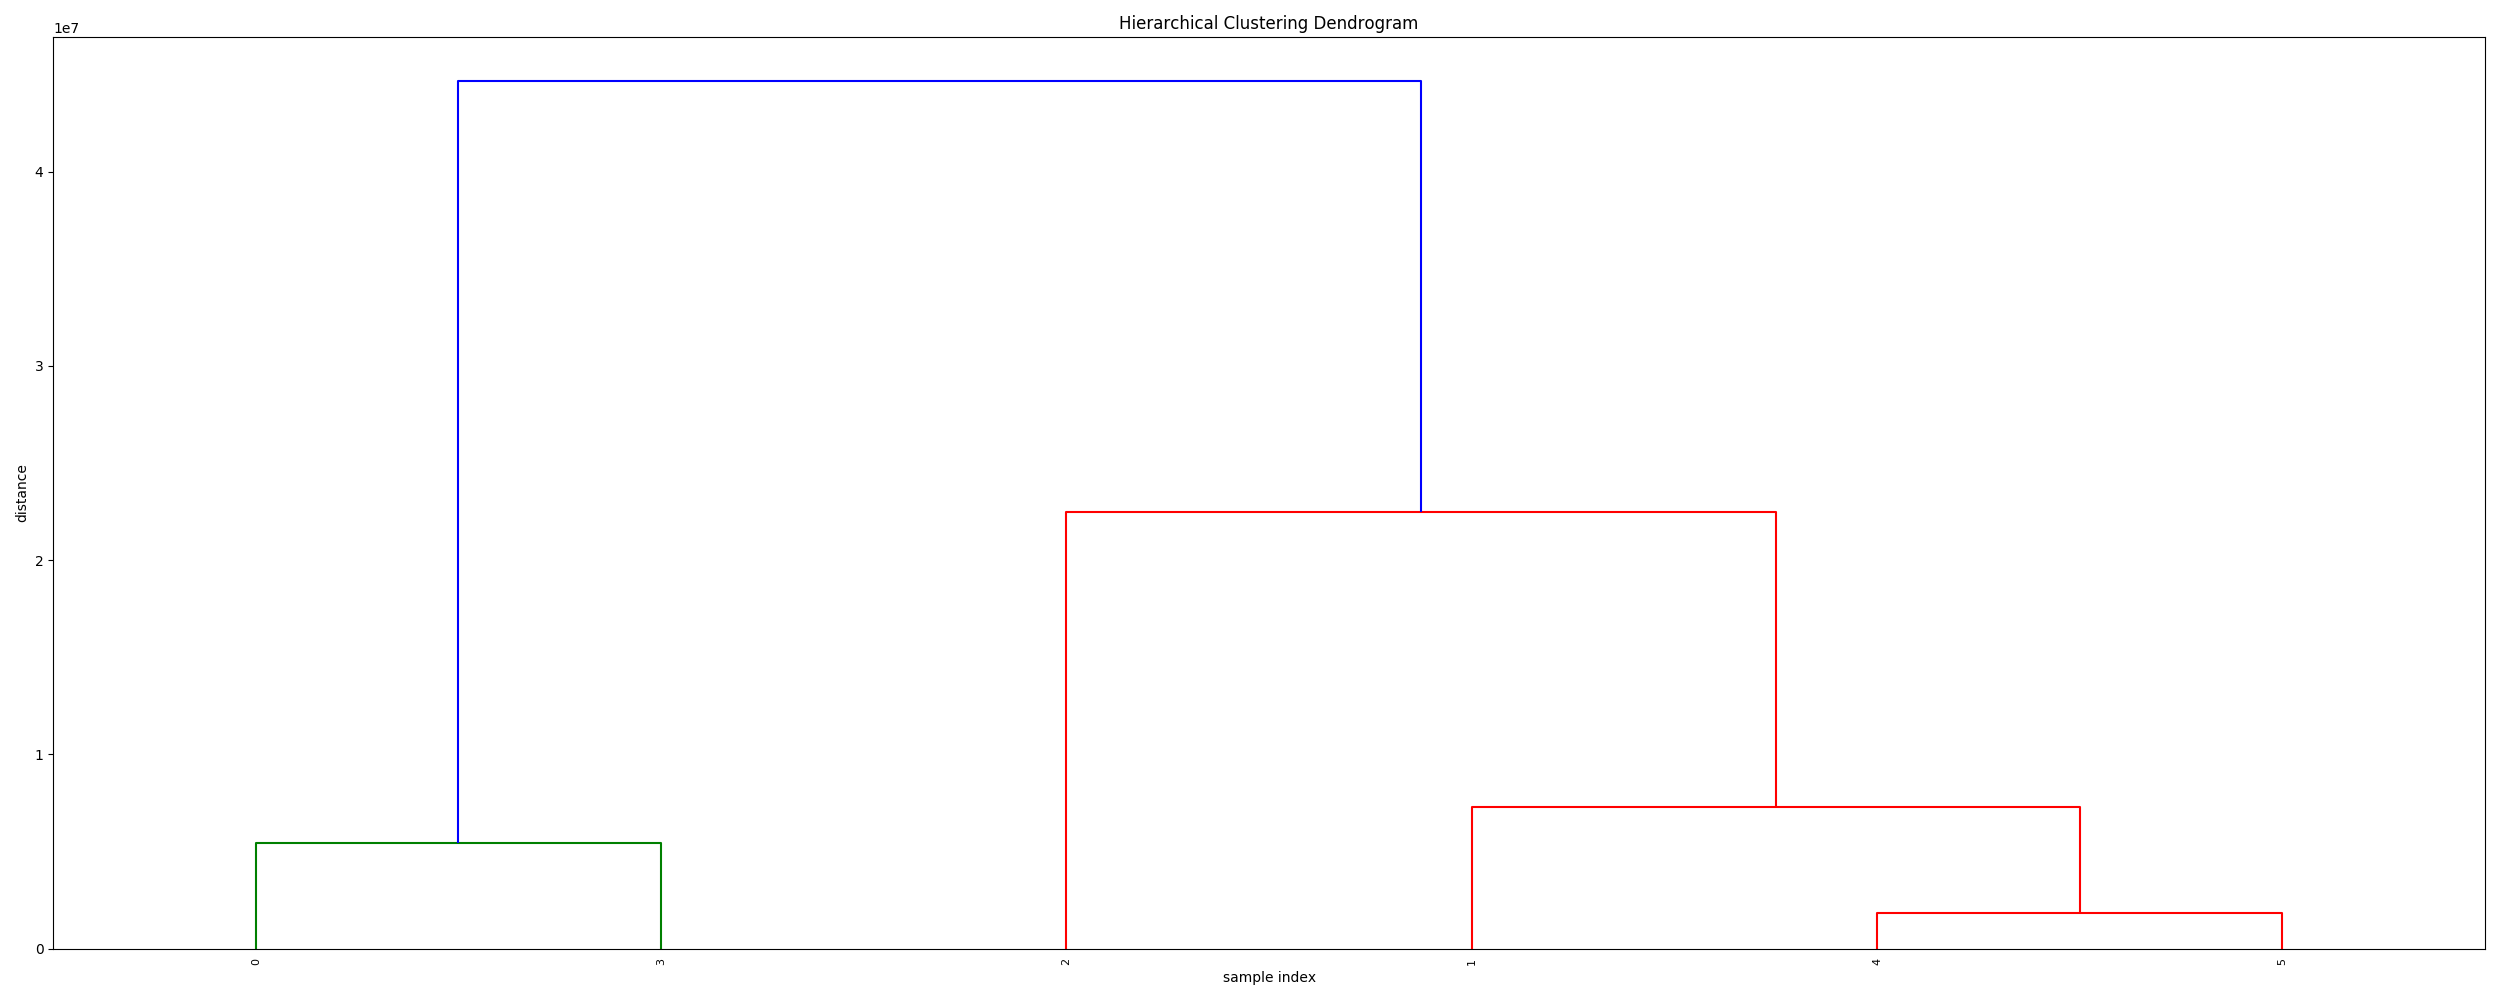
\includegraphics[width=\textwidth]{features_clusters.png}
        \caption{Clusters des premières séries}
        \label{fig:features_clusters}
    \end{figure}
\end{frame}

\begin{frame}
    \exemle{
        $\sum_{i=0}^{n}2^i$ donne \code{sum(2**i for i in range(n))}
    }
\end{frame}

\end{document}

